
\section{Introduction}
\section{Motivation}
\section{Matrix formulation of the problem - 1D interferometer}

Here I intend to use convolution matrices properties to {\it qualitatively} study how ``pseudo-PSF'' vary as a
function of source location. Here I limit myselves to a 1-dimensional
interferometer (scalar only), so that
Convolution matrices are Toeplitz-symetyric (see bellow). In a more
general case, (along my intuition - but should be thought more
carefully), convolution matrices should be block-Toeplitz (each
block is a Toeplitz), while symetricity should still be true. 

\subsection{Remarks on the convolution and linear algebra}

In functional form the convolution theorem can be written as follows:


\def\F{\mathcal{F}}
\def\Fm{\bm{F}}
\def\Gauss{\bm{\mathcal{G}}}
\def\conv{\mathcal{*}}

\begin{alignat}{2}
%\label{eq:Lin}
%\F \left{ a.b\right}=&\F \left{ a\right}.\F \left{b\right}\\
\F \left\{  a.b\right\}=& \F \left\{a\right\}\conv\F \left\{b\right\}
\end{alignat}

Noting the convolution product is linear, we can reexpress the
convolution product and associated theorem asing linear
transformations:

\newcommand{\C}[1]{\bm{\mathcal{C}}_{#1}}
\newcommand{\vv}[1]{\bm{#1}}
\def\one{\bm{1}}


\begin{alignat}{2}
\label{eq:ConvTh}
%\F \left{ a.b\right}=&\F \left{ a\right}.\F \left{b\right}\\
\Fm \vv{A}\vv{b}=& \C{\vv{A}}\Fm \vv{b}
\end{alignat}

\noindent where $\Fm$ is the Fourier operator of size 
$n_{uv}\times n_{lm}$ ($\Fm$ is unitary $\Fm^H\Fm=\one$), $\vv{b}$ is
a vector with size $n_{lm}$. The matrix $\vv{A}$ models the scalar
multiplication of each point in $\vv{b}$, and is therefore diagonal of
size $n_{lm}\times n_{lm}$, and $\C{\vv{A}}$ is the convolution matrix
of size $n_{uv}\times n_{uv}$. There is a bijective relation

\begin{alignat}{2}
\label{eq:ConvTh}
%\F \left{ a.b\right}=&\F \left{ a\right}.\F \left{b\right}\\
\vv{A} \longleftrightarrow \C{\vv{A}}
\end{alignat}
 
\noindent in the sense that a scalar multiplucation defines a convolution
function and conversely. The matrices $\vv{A}$ and $\C{\vv{A}}$ always
have the following properties:

\begin{itemize}
  \item $\vv{A}$ is diagonal

   \item In the 1D case
\begin{itemize}
  \item $\C{\vv{A}}$ is Toeplitz
  \item In addition, for radiointerferometry, because the uv plane is symetric, $\C{\vv{A}}$ is symetric
\end{itemize}

\end{itemize}

The matrix $\C{\vv{A}}$ being Toeplitz, each row $\left[ \C{\vv{A}}
  \right]_l$ with sky coordinate $l$ can be built using a
rolling operator $\Delta_l$ that shifts the first row (the PSF at the field
center for example) to location of row $l$:

\begin{alignat}{2}
\label{eq:ConvTh}
%\F \left{ a.b\right}=&\F \left{ a\right}.\F \left{b\right}\\
\left[ \C{\vv{A}} \right]_l =& \Delta_l \left\{ \left[ \C{\vv{A}} \right]_0 \right\}
and&\\
\left[ \C{\vv{A}} \right]_0 =& \Fm^H \ \text{diag}(\vv{A})
\end{alignat}

The rolling operator is essentially just a reindexing, and has the
following properties:

\begin{alignat}{2}
\label{eq:PropsDelta0}
%\F \left{ a.b\right}=&\F \left{ a\right}.\F \left{b\right}\\
\Delta_l \left\{ a\vv{x} \right\} =&  a \Delta_l \left\{\vv{x} \right\} \\
\label{eq:PropsDelta1}
\Delta_l \left\{ \sum_i \vv{x}_i \right\} =& \sum_i \Delta_l \left\{ \vv{x}_i \right\} 
\end{alignat}

\newcommand{\roll}[1]{\Delta_l \left\{#1\right\}}


\subsection{PSF behaviour}

If $\vv{X}$ is the true sky, then the dirty image $\vv{X}^D_{ij}$ of
baseline $(ij)$ can be written as:

\begin{alignat}{2}
\vv{x}^D_{ij} =& \Fm^H \vv{S}_{c,ij}  \C{\vv{T}} \vv{S}_{\square,ij} \Fm \vv{A} \vv{x}
\end{alignat}

\noindent where $\vv{A}_{ij}$ models the DDE effets and is an
$n_{pix}\times n_{pix}$ diagonal matrix (taking polarisation into
account it is an
$4n_{pix}\times 4n_{pix}$ block diagonal matrix), $\vv{T}$ is the tapering/averaging function, 
$\vv{S}_{\square}$ samples the region over which the
tapering/averaging is made, and $\vv{S}_{c,ij}$ selects the central point
of the averaged/tapered visibility set. Using Eq. \ref{eq:ConvTh}, we have:

\begin{alignat}{2}
\vv{x}^D_{ij} =&\ \C{\vv{S}_{c,ij}}  \vv{T} \C{\vv{S}_{\square,ij}}  \Fm^H \Fm \vv{A}_{ij} \vv{x}\\ 
 =&\  \C{\vv{S}_{c,ij}}  \vv{T} \C{\vv{S}_{\square,ij}}  \vv{A}_{ij}  \vv{x}\\ 
\label{eq:approx}
 \sim&\  \C{\vv{S}_{c,ij}}  \vv{T}    \vv{A}_{ij} \vv{x}
\end{alignat}

\noindent where Eq. \ref{eq:approx} is true when the support of the
function $T$ is smaller than the sampling domain of
$\vv{S}_{\square}$. 

Averaged over all baselines, the dirty image becomes:

\begin{alignat}{2}
\label{eq:PPSF}
\vv{x}^D =&\bm{\mathcal{C}}_{STA} \vv{x}\\
\text{with }\bm{\mathcal{C}}_{STA}=&\sum_{ij}  \C{\vv{S}_{c,ij}}  \vv{T}    \vv{A}_{ij}
\end{alignat}



\subsection{Deriving the Pseudo-PSF}

\subsubsection{PSF and Pseudo-PSF}

{\bf We can already see that $\C{\vv{S}_{c,ij}}
  \vv{T}    \vv{A}_{ij}$ in Eq. \ref{eq:approx} is NOT Toeplitz anymore
  because each colunm is multiplied by a different value (DDE
  muliplied by the tapering function). The dirty sky is therefore not
  anymore the convolution of the true sky by the psf} {\it ie} the PSF
varies accross the field of view.

\subsubsection{Slow way}

Calculate the psf estimating $\mathcal{C}$ from direct
calculation. Eventually at discrete locations on a grid.


\subsubsection{Quickly deriving the Pseudo-PSF}

This is tricky part. The problem amount to finding any column $l$ of
$\bm{\mathcal{C}}$ on demand. For notation convenience, we merge
$\vv{T}$ and $\vv{A}_{ij}$ together in $\vv{A}_{ij}$. Operator
$\left[\vec{M}\right]_l$ extracts column $l$ from matrix $\vec{M}$,
and using Eq. \ref{eq:PropsDelta0}, \ref{eq:PropsDelta1} and \ref{eq:PPSF}:

\begin{alignat}{2}
\left[\bm{\mathcal{C}}\right]_l =&
     \left[\sum_{ij}  \C{\vv{S}_{c,ij}}  \vv{A}_{ij}\right]_l\\
=& \sum_{ij} a^l_{ij} \left[\C{\vv{S}_{c,ij}}\right]_l \\
&\ \ \ \text{with } a^l_{ij}=\vv{A}_{ij}(l)\\
=& \sum_{ij} \roll{a^l_{ij} \left[\C{\vv{S}_{c,ij}}\right]_0} \\
=& \sum_{ij} \roll{\Fm^H a^l_{ij}\ \text{diag}\left(\vv{S}_{c,ij}\right) }
\end{alignat}

If we now assume that at any given location $l$, the scalar $a^l_{ij}$
can be described by a smooth {\it function} of the uv coordinates
($(ij)$-indices), then we can write:

\begin{alignat}{2}
\left[\bm{\mathcal{C}}\right]_l =
& \sum_{ij} \roll{ \Fm^H \vv{A}^l\ \text{diag}\left(\vv{S}_{c,ij}\right) }\\
=& \sum_{ij} \roll{\C{\vv{A}^l}\ \Fm^H \text{diag}\left(\vv{S}_{c,ij}\right) }\\
=& \sum_{ij} \roll{\C{\vv{A}^l}\ \left[\C{\vv{S}_{c,ij}}\right]_0 }\\
=& \roll{\C{\vv{A}^l}\ \sum_{ij} \left[\C{\vv{S}_{c,ij}}\right]_0 }\\
=& \roll{\C{\vv{A}^l}\ \left[\C{\vv{S}_{c}}\right]_0 }\\
\end{alignat}

The approximate observed Pseudo-PSF is the convolution of the PSF at
the phase center ($\left[\C{\vv{S}_{c}}\right]_0$) and the fourier transform of the uv-dependent tapering function at given
lm ($\C{\vv{A}^l}$).

In other words, to compute the PSF at a given location $(lm)$:

\begin{itemize}
  \item Find $\vv{A}$:
    \begin{itemize}
    \item Compute weight $w_{ij}$ for each baseline $(ij)$
    \item Fit the uv-dependent weight by (for example), a Gaussian function $w_{ij}\sim w(u,v)=\Gauss\left(u,v\right)$ 
    \end{itemize}
  \item Compute the $PSF_{lm}$ at $(lm)$ from the PSF at the phase center $PSF_0$ as $PSF_{lm}=\mathcal{F}^{-1}\left(w\right)\conv PSF_0$
\end{itemize}
For example if the long baselines are more tapered, they are
"attenuated". The effective PSF on the edge of the field will get
larger by the convolution...
Something like that...
\section{Numerical Experiments}
We demonstrate the computational complexity of the quick, the slow derived PSF as a function of sky coordinates and 
perform a direct numerical results.
\subsection{Slow derivation and computation cost}
\subsection{Quick derivation and computation cost}
We will now show how to derived a pseudo PSF  which is base and resolves on the nominal PSF
but labelled by a set of band-limited integration.
\subsubsection{Averaging case}
The approach is base on the  evaluation of the band limited case of the following infinite signal:
\begin{alignat}{2}
\tilde{s}(\kappa) =& \int_{-\infty}^{+\infty}exp(-j\kappa y)dy, \label{eq1111122}
\end{alignat}
where $\kappa$ is a real number and $\tilde{s}(\kappa)$ is the Fourier transform of a unitary function, $s(y)=1$. We can also see 
$\tilde{s}(\kappa)$ as a delta function, $\delta (\kappa)$.
If we band limited $\tilde{s}(\kappa)$ in a small finite phase range  $\Delta x_0$ centered on the phase $x_c$, Eq.\ref{eq11111} becomes:
\begin{alignat*}{2}
(B_{\Delta x_0}s)(x) =& \frac{1}{\Delta x_0}\int_{x_c-\frac{\Delta x_0}{2}}^{x_c+\frac{\Delta 
x_0}{2}}\tilde{s}(\kappa)exp(jx\kappa)d\kappa\label{eq1111111}\\
		     =& \frac{1}{\Delta x_0}\int_{x_c-\frac{\Delta x_0}{2}}^{x_c+\frac{\Delta x_0}{2}}\bigg( 
\int_{-\infty}^{+\infty}exp(-j\kappa y)dy\bigg)\\ 
		      & exp(jx\kappa)d\kappa\\
		     =&\int_{-\infty}^{+\infty}\bigg( \frac{1}{\Delta x_0} \int_{x_c-\frac{\Delta x_0}{2}}^{x_c+\frac{\Delta 
x_0}{2}}exp(j(x-y)\kappa)d\kappa\bigg)dy\\
		     =&\int_{-\infty}^{+\infty}K(x-y)dy\\
		     =& K(x)\circ s(x)\\
		     =&K(x)
\end{alignat*}
Where $s(x)=\mathcal{F}^{-1}\tilde{s}(\kappa)$ and,
\begin{alignat*}{2}
 K(x)=& \frac{1}{\Delta x_0} \int_{x_c-\frac{\Delta x_0}{2}}^{x_c+\frac{\Delta x_0}{2}}exp(jx\kappa )d\kappa\\
     =& sinc \big(x\frac{\Delta x_0}{2}\big) exp(jxx_c)
\end{alignat*}
Then the result follows:
\begin{alignat}{2}
(B_{\Delta x_0}s)(x) = & sinc \big(x\frac{\Delta x_0}{2}\big) exp(jxx_c). %\label{eq11avegcase}
\end{alignat}
% the phase in frequency $x_0=x_0(\nu)$
% Figure \ref{fig:amplitude_phase} shows that the averaged of sine functions can be approximate by a sinc function. Therefore, an approximate 
% of Eq\ref{eq:sines} is given as:
% \begin{alignat}{2}
% <s_{i}> \simeq sinc\frac{x_1}{2}exp(j\frac{x_2}{2})
% \end{alignat}
The result for a two dimensional case follows:
\begin{alignat}{2}
(B_{\Delta x_0 \Delta e_0}s)(x,e)=&sinc (x\frac{\Delta x_0}{2})sinc(e\frac{\Delta e_0}{2})\\
				  &exp\big(j (xx_c+ee_c)\big)
\end{alignat}
Prof:
\begin{alignat}{2}
\tilde{s}(\kappa,\gamma) =& \int_{-\infty}^{+\infty}\int_{-\infty}^{+\infty}exp\big(-j(\kappa y+\gamma h)\big)dydh, \label{eq2d}
\end{alignat}
where $\tilde{s}(\kappa,\gamma)=\delta(\kappa,\gamma)$. If the complex phase of  $\tilde{s}(\kappa,\gamma)$ varies linearly in time within 
the range $\Delta x_0$ centered on  $x_c$ and in frequency within the range
$\Delta e_0$ centered on $e_c$, then Eq.\ref{eq2d} becomes:\\
\begin{alignat*}{2}
(B_{\Delta x_0\Delta e_0}s)(x,e) =& \frac{1}{\Delta x_0\Delta e_0}\int_{x_c-\frac{\Delta x_0}{2}}^{x_c+\frac{\Delta 
x_0}{2}}\int_{e_c-\frac{\Delta e_0}{2}}^{e_c+\frac{\Delta e_0}{2}}\tilde{s}(\kappa,\gamma)\\
				  &exp(jx\kappa+je\gamma)d\kappa d\gamma\\
		     =& \frac{1}{\Delta x_0 \Delta e_0}\int_{-\infty}^{+\infty}\int_{x_c-\frac{\Delta x_0}{2}}^{x_c+\frac{\Delta 
x_0}{2}}exp\big(j\kappa(x-y)\big)\\
		      &d\kappa dy \bigg[\int_{-\infty}^{+\infty}\int_{e_c-\frac{\Delta e_0}{2}}^{e_c+\frac{\Delta 
e_0}{2}}exp\big(j\gamma(e-h)\big)d\gamma dh\bigg]\\
		     =&K_1(e)K_2(x)\\
		     =&sinc (x\frac{\Delta x_0}{2})sinc(e\frac{\Delta e_0}{2})exp\big(j (xx_c+ee_c)\big)
\end{alignat*}
We can therefore approximate averaging   by assuming that if $\Delta t$ and $\Delta \nu$ are
small enough that the amplitude of the visibility, $V_{pq}$ of a baseline $(p,q)$ remains constant while
the complex phase varies linearly in time and frequency. In a two dimensional case, the approximation then follows:
\begin{alignat}{2}
 V_{pq}^{avg}(t_c, \nu_c)\simeq& sinc\frac{\Delta \Psi}{2}sinc\frac{\Delta \Phi}{2} V_{pq}(t_{c},\nu_{c})\label{eq:visibility}.
\end{alignat}
Here, $\Delta \Psi$ and $\Delta \Phi$ are the phase changes in time and in frequency respectively, defined as:
\begin{alignat}{2}
\Delta \Phi=&arg V_{pq}(t_{c},\nu_{e})-arg V_{pq}(t_{c},\nu_{s})\\
\Delta \Psi=&arg V_{pq}(t_{e},\nu_{c})-arg V_{pq}(t_{s},\nu_{c})
\end{alignat}
The high resolution data $V_{pq}(t,\nu)$ that is been average is given by:
\begin{eqnarray}
 V_{pq}(t, \nu)=& exp\bigg\{2j\pi\big(u_{pq}l+v_{pq}m+ w_{pq}n\big)\bigg\}\label{eq233},
\end{eqnarray}
where, $u_{pq}$, $v_{pq}$ and $w_{pq}$ are the baseline coordinates that causes $V_{pq}$ to variate in time and frequency due to the Earth 
rotation.\\
% \begin{alignat}{2}
% u_{pq}=&u_{pq}(t,\nu)\\
% v_{pq}=&v_{pq}(t,\nu)\\
% w_{pq}=&w_{pq}(t,\nu)
% \end{alignat}
% 
% In this section, knowing the response of an array to a source at the phase centre $(l_0,m_0)$, we want to measure the array response at a 
% given location $(l,m)\neq(l_0,m_0)$.  A pair wise element $(p,q)$ of the array   measures the quantity at $(l,m)$:
% \begin{eqnarray}
%  V_{pq}(t, \nu)=& exp\bigg\{2j\pi\big(u_{pq}l+v_{pq}m+ w_{pq}n\big)\bigg\}\label{eq233},
% \end{eqnarray}
% where,
% \begin{alignat}{2}
% u_{pq}=&u_{pq}(t,\nu)\\
% v_{pq}=&v_{pq}(t,\nu)\\
% w_{pq}=&w_{pq}(t,\nu)
% \end{alignat}
% The Earth rotation causes $V_{pq}(t, \nu)$ to variate in time and  frequency. 
% Taking this effect into account, Eq. $\ref{eq233}$ is  rewritten as an integration over narrower time and frequency band. From the above 
% derivation, $x_0=x_0(t)$ and $y_0=y_0(\nu)$, we then have (coming directly from RIME1, Oleg):
% \begin{alignat}{2}
%  V_{pq}^{avg}(t_c, \nu_c)\simeq& sinc\frac{\Delta \Psi}{2}sinc\frac{\Delta \Phi}{2} V_{pq}(t_{c},\nu_{c})\label{eq:visibility},
% \end{alignat}
% where $t_{c}=\frac{t_{s} + t_{e}}{2}$, $\nu_{c}=\frac{\nu_{s} + \nu_{e}}{2}$ and 
% \begin{alignat}{2}
% \Delta \Phi=&arg V_{pq}(t_{c},\nu_{e})-arg V_{pq}(t_{c},\nu_{s})\\
% \Delta \Psi=&arg V_{pq}(t_{e},\nu_{c})-arg V_{pq}(t_{s},\nu_{c})
% \end{alignat}
The  results of the instrument averaged visibilities for all baselines then follows:
\begin{alignat}{2}
V(t,\nu)\simeq&\sum_{pq} V_{pq}^{avg}(t_c, \nu_c)\\
	\simeq&\sum_{pq} sinc\frac{\Delta \Psi}{2}sinc\frac{\Delta \Phi}{2} V_{pq}(t_{c},\nu_{c})\label{eq24}
\end{alignat}
For convenience let assume $V_{pq}(t_{c},\nu_{c})$ the visibility of a source at the phase centre (coordinates $(l_0,m_0)$) during the 
time $t_c$ at $\nu_c$. That said: 
\begin{eqnarray}
 V_{pq}(t_c, \nu_c)=& exp\bigg\{2j\pi\big(u_{pq}l_0+v_{pq}m_0+ w_{pq}n_0\big)\bigg\},
\end{eqnarray}
and $V_{pq}(t_{c},\nu_{e})$, $V_{pq}(t_{c},\nu_{s})$, $V_{pq}(t_{e},\nu_{c})$, $V_{pq}(t_{s},\nu_{c})$ the measurements data of a source 
locate at $(l,m)\neq(l_0,m_0)$ during $t_c$ at $\nu_e$, $t_c$ at $\nu_s$, $t_e$ at $\nu_c$ and  $t_s$ at $\nu_c$ respectively.\\
Eq\ref{eq24} is inverse Fourier transform and from the  convolution theorem, we have:
\begin{alignat}{2}
R(l,m)\simeq& \sum_{pq}\mathcal{F}^{-1}\bigg\{sinc\frac{\Delta \Psi}{2}sinc\frac{\Delta \Phi}{2}\bigg\}\\
	\circ& R_{pq}(l_0,m_0).
\end{alignat}
Here, $R(l,m)$ is the instrument response (PSF) for a source at location $(l,m)$ and $R_{pq}(l_0,m_0)$ the response of the baseline 
$(p,q)$ for a source at the phase centre.\\
Assuming that all the baselines are pointing at the same phase centre then the previous becomes:
\begin{alignat}{2}
R(l,m)\simeq&\bigg(\sum_{pq}\mathcal{F}^{-1}\bigg\{sinc\frac{\Delta \Psi}{2}sinc\frac{\Delta \Phi}{2}\bigg\}\bigg)
	\circ& R_{}(l_0,m_0)\\
      \simeq& Tri(l,m)\circ R(l_0,m_0).\label{eqtota}
\end{alignat}
With, $R(l_0,m_0)$ the instrument response for a source at the phase centre and the function, $Tri(l,m)$ is defined as:
\begin{equation*}
Tri(l,m)=\left\{
\begin{array}{rl}
a_{lm}\neq 1 & \mbox{if (l,m) exist} \\
0 & \mbox{otherwise}
\end{array}\right.
\end{equation*}
\subsubsection{General case}
From our previous work, we showed that averaging is similar to convolving the visibilities with a top-hat function, then we 
furthermore replaced the top-hat function by a function, $f_w$. With our terminology, if we tape the visibilities with a function $f_w$, a 
general case of  Eq. $\ref{eq1111122}$ is derived as follows:
\begin{alignat}{2}
\tilde{s}(\kappa) =& \int_{-\infty}^{+\infty}f_{w}(y)exp(-j\kappa y)dy \label{eq:genral} \\
       % =& exp(jx_c)\int_{-\infty}^{+\infty}f_{b}(u)exp(ju)du\\
        %=& exp(jx_c)F_b(x_0)\label{eq11115}
\end{alignat}
In this case, $\tilde{s}(\kappa)$ is the Fourier transform of $f_w(\kappa)$. Following the derivation of Eq.\ref{eqavegcase}, a general 
case of the band-limited form of Eq.\ref{eq:genra} is:
% \begin{alignat*}{2}
% (B_{\Delta x_0}s)(x) =& \frac{1}{\Delta x_0}\int_{x_c-\frac{\Delta x_0}{2}}^{x_c+\frac{\Delta 
% x_0}{2}}\tilde{s}(\kappa)exp(jx\kappa)d\kappa\label{eq1111111}\\
% 		     =& \frac{1}{\Delta x_0}\int_{x_c-\frac{\Delta x_0}{2}}^{x_c+\frac{\Delta x_0}{2}}\bigg( 
% \int_{-\infty}^{+\infty}f_b(y)exp(-j\kappa y)dy\bigg)\\ 
% 		      & exp(jx\kappa)d\kappa\\
% 		     =&\int_{-\infty}^{+\infty}f_b(y)\bigg(\frac{1}{\Delta x_0} \int_{x_c-\frac{\Delta x_0}{2}}^{x_c+\frac{\Delta 
% x_0}{2}}exp(j(x-y)\kappa)d\kappa\bigg)dy\\
% 		     =&\int_{-\infty}^{+\infty}K(x-y)f_b(y)dy\\
% 		     =& K(x)\circ f_b(x)
% \end{alignat*}
%Then the result follows:
\begin{alignat*}{2}
(B_{\Delta x_0}s)(x) = & \bigg[sinc \big(x\frac{\Delta x_0}{2}\big) exp(jxx_c)\bigg]\circ f_w(x)\\
		     = & \bigg[sinc \big(x\frac{\Delta x_0}{2} \big)\circ f_w(x)\bigg]exp(jxx_c)
\end{alignat*}
In a two dimensional case, the previous becomes:
\begin{alignat*}{2}
(B_{\Delta x_0 \Delta e_0}s)(x,e)=&\bigg[sinc (x\frac{\Delta x_0}{2})sinc(e\frac{\Delta e_0}{2})\circ f_{w}(x,e)\bigg]\\
				  &exp\big(j (xx_c+ee_c)\big)
\end{alignat*}
Eq.\ref{eq:visibility} can therefore be estimate in a general case as:
\begin{alignat}{2}
 V_{pq}^{corr}(t_c, \nu_c)\simeq& \bigg[sinc\frac{\Delta \Psi}{2}sinc\frac{\Delta \Phi}{2}\circ f_{w}(t_c,\nu_c)\bigg]
			   V_{pq}(t_{c},\nu_{c})
\end{alignat}
The  results of the instrument weighted average visibilities for all baselines then follows:
\begin{alignat}{2}
R(l,m)\simeq& \sum_{pq}\mathcal{F}^{-1}\bigg\{sinc\frac{\Delta \Psi}{2}sinc\frac{\Delta \Phi}{2}\circ f_{w}(t_c,\nu_c)\bigg\}\\
	\circ& R_{pq}(l_0,m_0)\\
	\simeq& \sum_{pq}\mathcal{F}^{-1}\bigg\{sinc\frac{\Delta \Psi}{2}sinc\frac{\Delta 
\Phi}{2}\bigg\}\mathcal{F}^{-1}\bigg\{f_{w}(t_c,\nu_c)\bigg\}\\
	\circ& R_{pq}(l_0,m_0)\\
	\simeq& \bigg[Tri(l,m)F_{w}(l_0,m_0)\bigg]\circ R(l_0,m_0),
\end{alignat}
where $\mathcal{F}^{-1}\bigg\{f_{w}(t_c,\nu_c)\bigg\}=F_{w}(l_0,m_0)$.
% \begin{alignat}{2}
% \Delta \Psi\simeq& \Delta \Phi
% \end{alignat}
% % \begin{figure*}
% % \begin{minipage}{0.38\linewidth}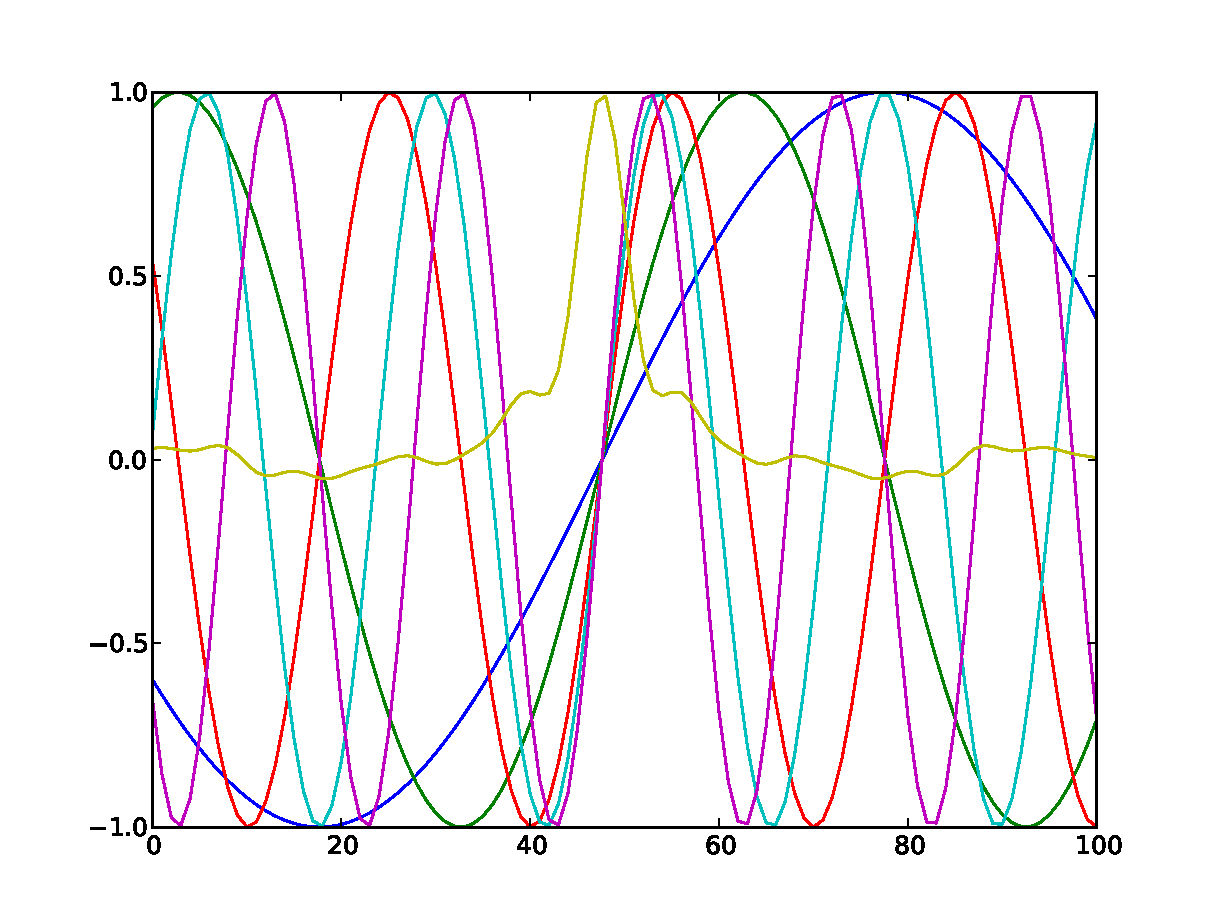
\includegraphics[width=1\textwidth]{./Figures/amplitude_phase.pdf}\caption{averages sine 
% % functions vs. sinc function}\label{fig:amplitude_phase}
% % \end{minipage}
%   \hspace{1cm} 
% \begin{minipage}{0.38\linewidth}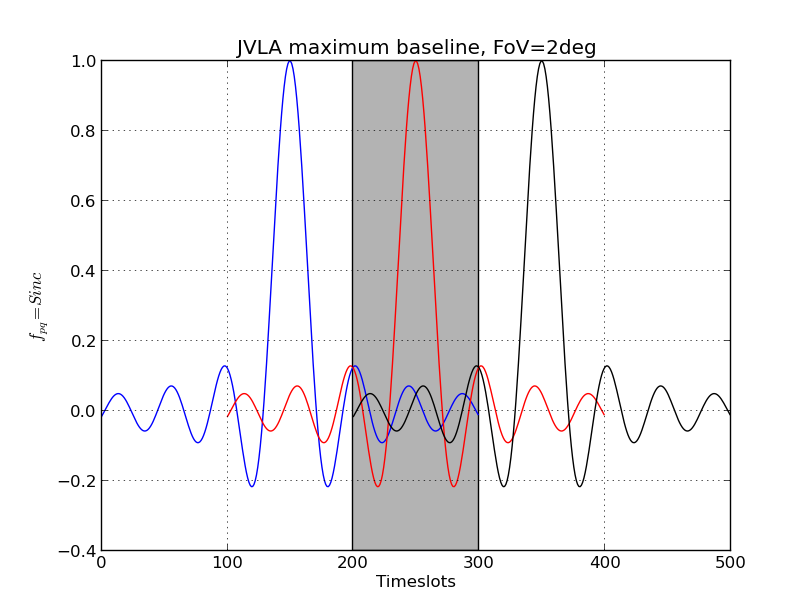
\includegraphics[width=1\textwidth]{./Figures/corrSigVLAMxBl_overlapGdelta.pdf}\caption{Overlap 
% baseline dependent windowing functions}\label{fig:corrSigVLAMxBl_overlapGdelta}\end{minipage}
%\end{figure*}
\section{Simulation and comparison}
\section{Discussion and conclusion}